\chapter{Analyse der künstlichen neuronalen Netze}

Die Banken - und Finanzkrise der letzten Jahre beherrschte die Gedanken von Anlegern, Sparern, Investoren, Volk und Politikern. Als Startzeitpunkt kann der 9. August 2007 gesehen werden, wobei bis heute Auswirkungen im Finanzsystem zu spüren sind und kein klarer Endzeitpunkt, auch auf Grund der globalen Reichweite, festgemacht werden. Eines ist klar, lineare Zusammenhänge zwischen Börsenkursen können in einer solch einer Extremsituation ausgeschlossen werden. Dieses Kapitel hat nicht nur entscheidende Zeiträume dieser Finanzkrise im Bezug auf die Vorhersagegenauigkeit von Börsenkursschlusswerten untersucht, sondern auch den Zeitraum in dem der Vorfall des Kernkraftwerks in Fukushima statt fand, betrachtet.

\begin{minipage}[c]{0.5\textwidth}

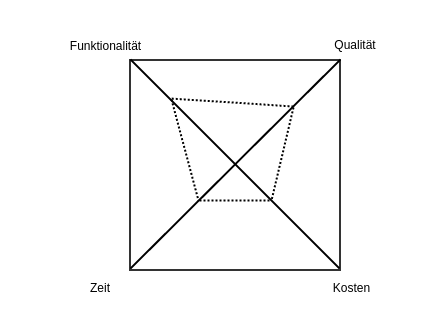
\includegraphics[width=0.49\textwidth]{Bilder/Konzeption/mag_viereck_not_linear.png}
\captionof{figure}{Abb - nicht lineare}

\end{minipage}
\begin{minipage}[c]{0.5\textwidth}
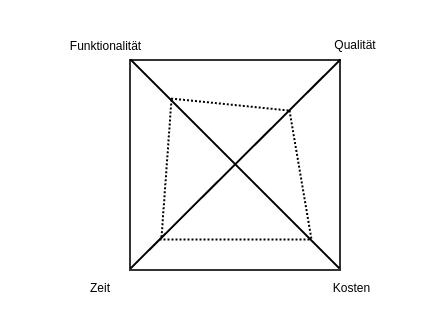
\includegraphics[width=0.49\textwidth]{Bilder/Konzeption/mag_viereck_linear.png}
\captionof{figure}{Abb - lineare}
\end{minipage}  